\chapter{Architecture}\label{ch:architecture}

The aim for this project is to design and implement a cloud-based task submission and execution system with elasticity requirements.
This involves using Google Cloud Platform~\cite{google-cloud-platform} services for storage, communication, and computation.


\section{System Overview}\label{sec:system-overview}

The system, denotated \texttt{VisionFlow},
was designed to detect features/characteristics (e.g., tree, street, cat)
in image files (JPG, PNG, etc.) and translate these features, commonly known as labels, from English to another language.

Without entering into the details, the system overview is depicted in Figure~\ref{fig:system-architecture}.

\begin{figure}[!htb]
    \centering
    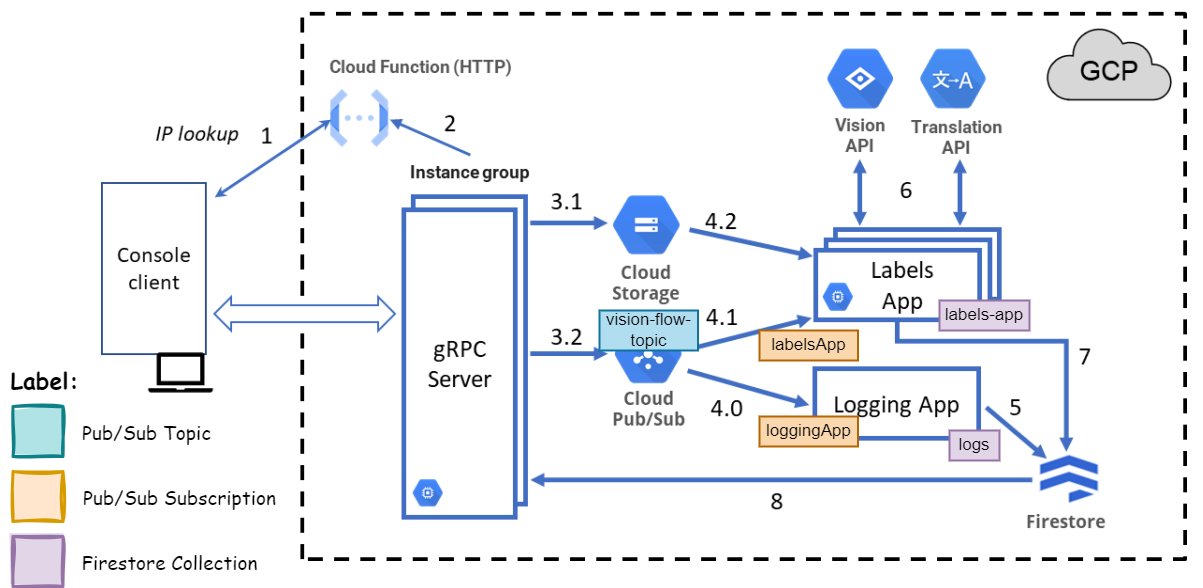
\includegraphics[width=1\textwidth]{../figures/system-architecture}
    \caption{System Overview}
    \label{fig:system-architecture}
\end{figure}


\section{Description}\label{sec:system-description}

The system is composed of the following components:

\begin{itemize}
    \item \textbf{Client}:
    Application responsible for submitting operations to the server after establishing a connection using a lookup service;
    \item \textbf{Server}: Responsible for handling requests from the client and orchestrating the processing of image files;
    \item \textbf{Google Cloud Storage}: Cloud object storage used to store the image files that are submitted by the client as blobs;
    \item \textbf{Google Cloud Pub/Sub}: Messaging service used to notify the image processing applications that a new image file is available for processing;
    \item \textbf{Google Cloud HTTP Function}: Serveless function used by the client to fetch the IP addresses of running server instances within a specified instance group;
    \item \textbf{Google Cloud Compute Engine}: Orchestration and monitoring service used to manage the instance groups of the server and the image processing application;
    \item \textbf{Google Cloud Vision}: Cloud service used to detect features in image files;
    \item \textbf{Google Cloud Translation}: Cloud service used to translate the detected features from English to another language;
    \item \textbf{Firestore}: Serveless NoSQL document database used to store the processed information of the image files.
\end{itemize}
